%------------------------------------------------------------------------
%Editar Diplomado
\hypertarget{cv:eliminarActor}{\section{Eliminar Actor}} \label{sec:eliminarActor}

	Esta funcionalidad le permitirá eliminar un actor innecesaria o incorrecta. Para eliminar un actor es necesario que no se encuentre asociado a casos de uso.

		\subsection{Procedimiento}

			%Pasos de procedimiento
			\begin{enumerate}
	
			\item Oprima el botón \IUBotonEliminar{} de un registro existente de la pantalla \ref{fig:GestionarActores} ''Gestionar Actores''.
	
			\item Se mostrará el mensaje \ref{fig:confirmaEliminaActor} sobre la pantalla \ref{fig:GestionarActores} ''Gestionar Actores''.
			
			%Pantalla
			\begin{figure}[htbp!]
				\begin{center}
					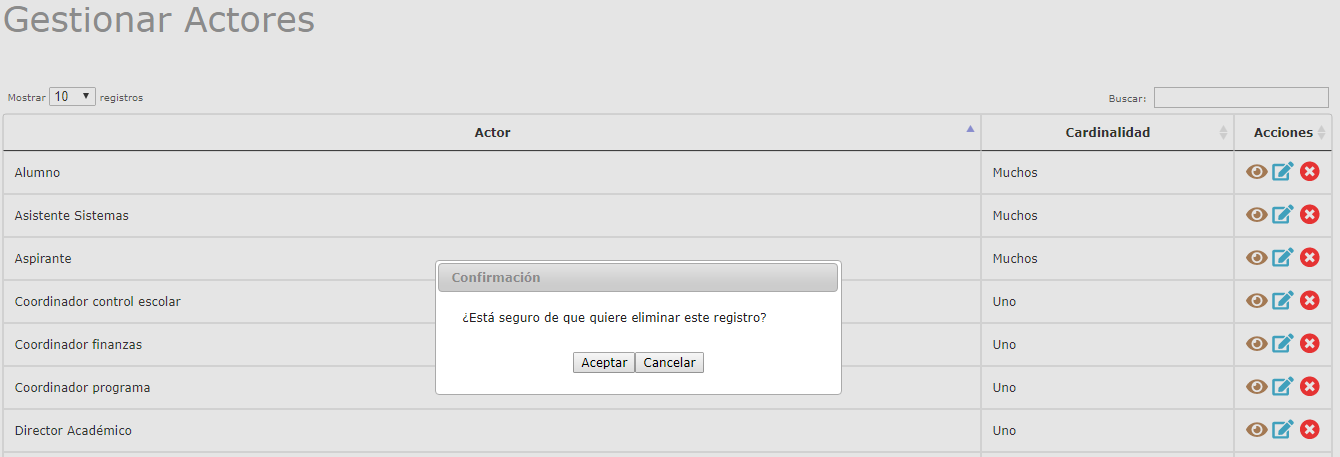
\includegraphics[scale=0.5]{roles/lider/actor/pantallas/IU10-3MSG10}
					\caption{MSG de Confirmación}
					\label{fig:confirmaEliminaActor}
				\end{center}
			\end{figure}
						
			\item Oprima el botón \IUAceptar.
			
			\item Se mostrará el mensaje \ref{fig:actorEliminado} en la pantalla \ref{fig:GestionarActores} ''Gestionar Actores''.
			
			\begin{figure}[htbp!]
				\begin{center}
					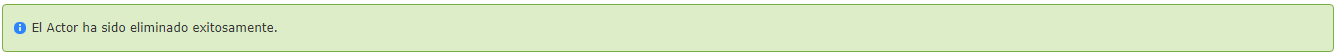
\includegraphics[scale=0.5]{roles/lider/actor/pantallas/IU10-3MSG1}
					\caption{MSG: Actor Eliminado}
					\label{fig:actorEliminado}
				\end{center}
			\end{figure}
			\end{enumerate}